% --------------------------------------------------------------
% This is all preamble stuff that you don't have to worry about.
% Head down to where it says "Start here"
% --------------------------------------------------------------
 
\documentclass[12pt]{article}
 
\usepackage[margin=1in]{geometry} 
\usepackage{amsmath,amsthm}
 
\usepackage{graphicx}
\graphicspath{ {./img/} }

\usepackage{tikz}

\usepackage{amssymb}

\usepackage{listings}
\usepackage{color}
 
\definecolor{codegreen}{rgb}{0,0.6,0}
\definecolor{codegray}{rgb}{0.5,0.5,0.5}
\definecolor{codepurple}{rgb}{0.58,0,0.82}
\definecolor{backcolour}{rgb}{0.95,0.95,0.92}
 
\lstdefinestyle{mystyle}{
    backgroundcolor=\color{backcolour},   
    commentstyle=\color{codegreen},
    keywordstyle=\color{magenta},
    numberstyle=\tiny\color{codegray},
    stringstyle=\color{codepurple},
    basicstyle=\footnotesize,
    breakatwhitespace=false,         
    breaklines=true,                 
    captionpos=b,                    
    keepspaces=true,                 
    numbers=left,                    
    numbersep=5pt,                  
    showspaces=false,                
    showstringspaces=false,
    showtabs=false,                  
    tabsize=2
}
 
\lstset{style=mystyle}

\let\oldemptyset\emptyset
\let\emptyset\varnothing

\newcommand{\N}{\mathbb{N}}
\newcommand{\Z}{\mathbb{Z}}
 
\newenvironment{theorem}[2][Theorem]{\begin{trivlist}
\item[\hskip \labelsep {\bfseries #1}\hskip \labelsep {\bfseries #2.}]}{\end{trivlist}}
\newenvironment{lemma}[2][Lemma]{\begin{trivlist}
\item[\hskip \labelsep {\bfseries #1}\hskip \labelsep {\bfseries #2.}]}{\end{trivlist}}
\newenvironment{exercise}[2][Exercise]{\begin{trivlist}
\item[\hskip \labelsep {\bfseries #1}\hskip \labelsep {\bfseries #2.}]}{\end{trivlist}}
\newenvironment{reflection}[2][Reflection]{\begin{trivlist}
\item[\hskip \labelsep {\bfseries #1}\hskip \labelsep {\bfseries #2.}]}{\end{trivlist}}
\newenvironment{proposition}[2][Proposition]{\begin{trivlist}
\item[\hskip \labelsep {\bfseries #1}\hskip \labelsep {\bfseries #2.}]}{\end{trivlist}}
\newenvironment{corollary}[2][Corollary]{\begin{trivlist}
\item[\hskip \labelsep {\bfseries #1}\hskip \labelsep {\bfseries #2.}]}{\end{trivlist}}
\newenvironment{question}[2][Question]{\begin{trivlist}
\item[\hskip \labelsep {\bfseries #1}\hskip \labelsep {\bfseries #2.}]}{\end{trivlist}}
\newenvironment{answer}[2][Answer]{\begin{trivlist}
\item[\hskip \labelsep {\bfseries #1}\hskip \labelsep {\bfseries #2.}]}{\end{trivlist}}

 
\begin{document}

% --------------------------------------------------------------
%                         Start here
% --------------------------------------------------------------

%\renewcommand{\qedsymbol}{\filledbox}

\newcommand{\coliumbrella}[7]{
	\begin{tikzpicture}[]
		\path (0,5) node(l) {#4}
		(3,5) node(m) {#5}
		(6,5) node(r) {#6}
		(3,8) node(t) {#1}
		(1.5,6) node(lt) {#2}
		(4.5,6) node(rt) {#3}
		(3,2) node(b) {#7};
		\draw (b) -- (l)
		(b) -- (r)
		(b) -- (m)
		(l) .. controls (1,6) and (2,6) .. (m)
		(m) .. controls (4,6) and (5,6) .. (r)
		(l) .. controls (2,8) and (4,8) .. (r);
	\end{tikzpicture}
}

\title{Assignment 4}%replace X with the appropriate number
\author{Michael Lee\\ %replace with your name
	CCST9017 - Hidden Order in Daily Life: A Mathematical Perspective \\
	University Number 3035569110 \\
	Tutorial Group 009
} %if necessary, replace with your course title

\maketitle

\begin{question}{1a}
	Model the situation as a suitable cooperative game (N; v).
\end{question}
\begin{answer}{1a}\end{answer}
Let Amy, Betty and Clara be player 1, 2 and 3 respectively \\
Hence $N=\{1,2,3\}$ \\
Such model should be
\begin{flalign*}
	v(\emptyset) & =0       &\\
	v(1)         & =125     &\\
	v(2)         & =130     &\\
	v(3)         & =200     &\\
	v(1,2)       & =125+130 &\\
	& =255     &\\
	v(2,3)       & =130+200 &\\
	& =330     &\\
	v(1,3)       & =125+200 &\\
	& =325 &\\
	v(1,2,3) &=350&
\end{flalign*}

\begin{question}{1b}
	Use a diagram to represent the game defined in part a
\end{question}

\begin{answer}{1b}\end{answer}
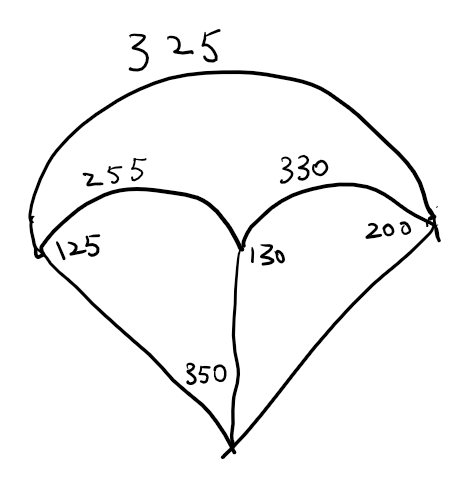
\includegraphics[scale=0.5]{hku-ccst9017-assignment-4-img-001}
\coliumbrella {$325$} {$255$} {$330$} {$125$} {$130$} {$200$} {$350$}

\begin{question}{1c}
	Find the Shapley value of the game by using two different methods.
\end{question}

\begin{answer}{1c}
	First method: Spliting game
\end{answer}
\coliumbrella {$325$} {$255$} {$330$} {$125$} {$130$} {$200$} {$350$} \\
$=$\coliumbrella {$125$} {$125$} {$0$} {$125$} {$0$} {$0$} {$125$}
$+$\coliumbrella {$0$} {$130$} {$130$} {$0$} {$130$} {$0$} {$130$} \\
$+$\coliumbrella {$200$} {$0$} {$200$} {$0$} {$0$} {$200$} {$200$}
$+$\coliumbrella {$0$} {$0$} {$0$} {$0$} {$0$} {$0$} {$-105$} \\ \\
After the split, we can obtain the Shapley value of the game with
\begin{align*}
	  & ( & 125 & , & 0   & , & 0   & ) \\
	+ & ( & 0   & , & 130 & , & 0   & ) \\
	+ & ( & 0   & , & 0   & , & 200 & ) \\
	+ & ( & -35 & , & -35 & , & -35 & ) \\
	= & ( & 90  & , & 95  & , & 165 & )
\end{align*}
Hence the Shapley value of this game is $(90,95,165)$ \\

\begin{answer}{1c}
	Second method: Applying Shapley’s Formula
\end{answer}
To faciliate computation, I uses a Python script as shown below.
\lstinputlisting[language=Python]{./src/q1-shapley.py}
As the result of computation, it is verified that the Shapley value of this game is $(90,95,165)$ \\
Therefore, with $90+95+165=350$, Amy, Betty and Clara should earn \$90, \$95 and \$165 respectively. \\

\begin{question}{2a}
	Model this situation as a game in coalitional form (N;v), where N={1,2,3} and v is the cost function.
\end{question}
\begin{answer}{2a}\end{answer}
Let town A, B and C be player 1, 2 and 3 respectively, \\
cost function $v(S)$ is in a unit of million \\
Hence $N=\{1,2,3\}$ \\
Such model should be
\begin{flalign*}
	v(\emptyset) & =0       &\\
	v(1)         & =12     &\\
	v(2)         & =6     &\\
	v(3)         & =8     &\\
	v(1,2)       & =15 &\\
	v(2,3)       & =11 &\\
	v(1,3)       & =17 &\\
	v(1,2,3)     & =20 &
\end{flalign*}

\begin{question}{2b}
	Assume the grand coalition N is formed. Find the Shapley value of the game by splitting the game into some suitable games.
\end{question}
\begin{answer}{2b}
	Splitting the game below.
\end{answer}
\coliumbrella {$17$} {$15$} {$11$} {$12$} {$6$} {$8$} {$20$} \\
$=$\coliumbrella {$0$}  {$6$}  {$6$}  {$0$}  {$6$} {$0$} {$6$}
$+$\coliumbrella {$8$}  {$0$}  {$8$}  {$0$}  {$0$} {$8$} {$8$} \\
$+$\coliumbrella {$12$} {$12$} {$0$}  {$12$} {$0$} {$0$} {$12$}
$+$\coliumbrella {$-3$} {$0$}  {$0$}  {$0$}  {$0$} {$0$} {$-3$} \\
$+$\coliumbrella {$0$}  {$-3$} {$0$}  {$0$}  {$0$} {$0$} {$-3$}
$+$\coliumbrella {$0$}  {$0$}  {$-3$} {$0$}  {$0$} {$0$} {$-3$} \\
$+$\coliumbrella {$0$}  {$0$}  {$0$}  {$0$}  {$0$} {$0$} {$3$} \\

After the split, we can obtain the Shapley value of the game with
\begin{align*}
	  & ( & 0    & , & 6    & , & 0    & ) \\
	+ & ( & 0    & , & 0    & , & 8    & ) \\
	+ & ( & 12   & , & 0    & , & 0    & ) \\
	+ & ( & -1.5 & , & 0    & , & -1.5 & ) \\
	+ & ( & -1.5 & , & -1.5 & , & 0    & ) \\
	+ & ( & 0    & , & -1.5 & , & -1.5 & ) \\
	+ & ( & 1    & , & 1    & , & 1    & ) \\
	= & ( & 10   & , & 4    & , & 6    & )
\end{align*}
Hence the Shapley value of this game is $(10,4,6)$ \\

\begin{question}{2c}
	Suppose A’s cost is decreased from $12 million to $11 million and all the other costs are unchanged. Find the new Shapley value of the game.
\end{question}
\begin{answer}{2c}\end{answer}
The new model should be
\begin{flalign*}
	v(\emptyset) & =0       &\\
	v(1)         & =11     &\\
	v(2)         & =6     &\\
	v(3)         & =8     &\\
	v(1,2)       & =15 &\\
	v(2,3)       & =11 &\\
	v(1,3)       & =17 &\\
	v(1,2,3)     & =20 &
\end{flalign*}
To faciliate computation, I modified the Python script to as shown below.
\lstinputlisting[language=Python]{./src/q2-shapley.py}
The new Shapley value of this game is $(9\frac 2 3,4\frac 1 6,6\frac 1 6)$ \\
% --------------------------------------------------------------
%     You don't have to mess with anything below this line.
% --------------------------------------------------------------

\end{document}